\documentclass[]{article}
\usepackage{graphicx}
%opening
\title{CLRS Exercise}
\author{Tongda Xu}

\begin{document}

\maketitle
\section{7}
\subsection{7.3}
\subsubsection{a}
This is certain concerning the $Randomized$ procedure, the probability of any index $i$ is chosen from $[0,n-1]$is:\\
$Pr(pivot = i) = \frac{1}{n}$\\
$E(X_{i}) = 1*Pr(pivot = i) + 0*Pr(pivot \neq i) = \frac{1}{n}$

\subsubsection{b}
It is certain that if $ith$ element is chosen as pivot, $Random-Parition$ cost $\Theta(n)$ time, and it will call $QuickSort[1, q-1], QuickSort[q+1, n]$ recursively.\\
Concerning only the first $Parition$, this would be the result:\\
$E(T(n)) = \Sigma_{i=1}^{n}Pr(pivot = i)(T(i-1) + T(n-i) + \Theta(n))\\
 = \Sigma_{i=1}^{n}X_{i}(T(i-1) + T(n-i) + \Theta(n))$
 
\subsubsection{c}
Concerning $X_{i} = \frac{1}{n}\\
E(T(n)) = \Sigma_{i=1}^{n}\frac{1}{n}(T(i-1) + T(n-i) + \Theta(n))\\
= \Sigma_{i=1}^{n}\frac{1}{n}T(i-1) + \Sigma_{i=1}^{n}\frac{1}{n}T(n-i) + \Sigma_{i=1}^{n}\frac{1}{n}\Theta(n)\\
= \frac{2}{n}\Sigma_{i=1}^{n-1}T(i) + \Theta(n)$

\subsubsection{d}
$\Sigma_{k=2}^{n-1}klgk \\
\le lg\frac{n}{2}\Sigma_{k=2}^{\frac{n}{2}}k + lgn\Sigma_{k=\frac{n}{2}}^{n-1}k\\
= lgn\Sigma_{k=2}^{n-1}k - lg2\Sigma_{k=2}^{\frac{n}{2}}k\\
= lgn\frac{(n+1)(n-2)}{2} - \frac{(\frac{n}{2} + 2)(\frac{n}{2}-1)}{2}\\
\le lgn\frac{n^2}{2} - \frac{n^2}{8}$\\
by Calculus, we have:\\
$(\frac{1}{2}x^2lgx - \frac{1}{4}x^2)|_{1}^{n-1} \le E(T(n)) \le (\frac{1}{2}x^2lgx - \frac{1}{4}x^2)|_{2}^{n}$

\subsubsection{e}
Proof of $E(T(n)) = O(nlgn)$:\\
Assume that $\forall k \in [1, n-1], \exists c, E(T(k)) \le cklgk - \Theta(k)$\\
For $k = n, E(T(n)) \le \frac{n}{2}c(lgn\frac{n^2}{2} - \frac{n^2}{4} - \Theta (n^2)) + \Theta(n) \le cnlgn - \Theta(n) $\\
Proof of $E(T(n)) =\Omega(nlgn)$:\\
Assume that $\forall k \in [1, n-1], \exists c, E(T(k)) \ge cklgk + \Theta(k)$\\
For $k = n, E(T(n)) \ge \frac{n}{2}c(lgn\frac{(n-1)^2}{2} - \frac{(n-1)^2}{4} + \Theta(n^2)) + \Theta(n) \ge cnlgn + \Theta(n)$\\
$\rightarrow E(T(n)) = \Theta(nlgn)$
\section{15}

\subsection{15.1-1}
$2^n -1 = \Sigma_{j = 0}^{n-1} 2^j $
\subsection{15.1-2}
Do not know how!

\subsection{15.1-3}
See Code

\subsection{15.1-4}
See Code

\subsection{15.1-5}
See Code

\subsection{15.2-1}
See Code

\subsection{15.2-2}
See Code

\subsection{15.2-3}

Assume that $\forall k \le n-1, T(k) \ge c2^k$\\
Then $T(n) = \Sigma_{k = 1}^{n-1} T(k)T(n-k) = (n-1)c^22^n > c2^n$\\
So $T(n) = \Omega (n), \omega(n)$

\subsection{15.2-4}
See Figure ~\ref{fig:15.2-4}

\begin{figure}
	\centering
	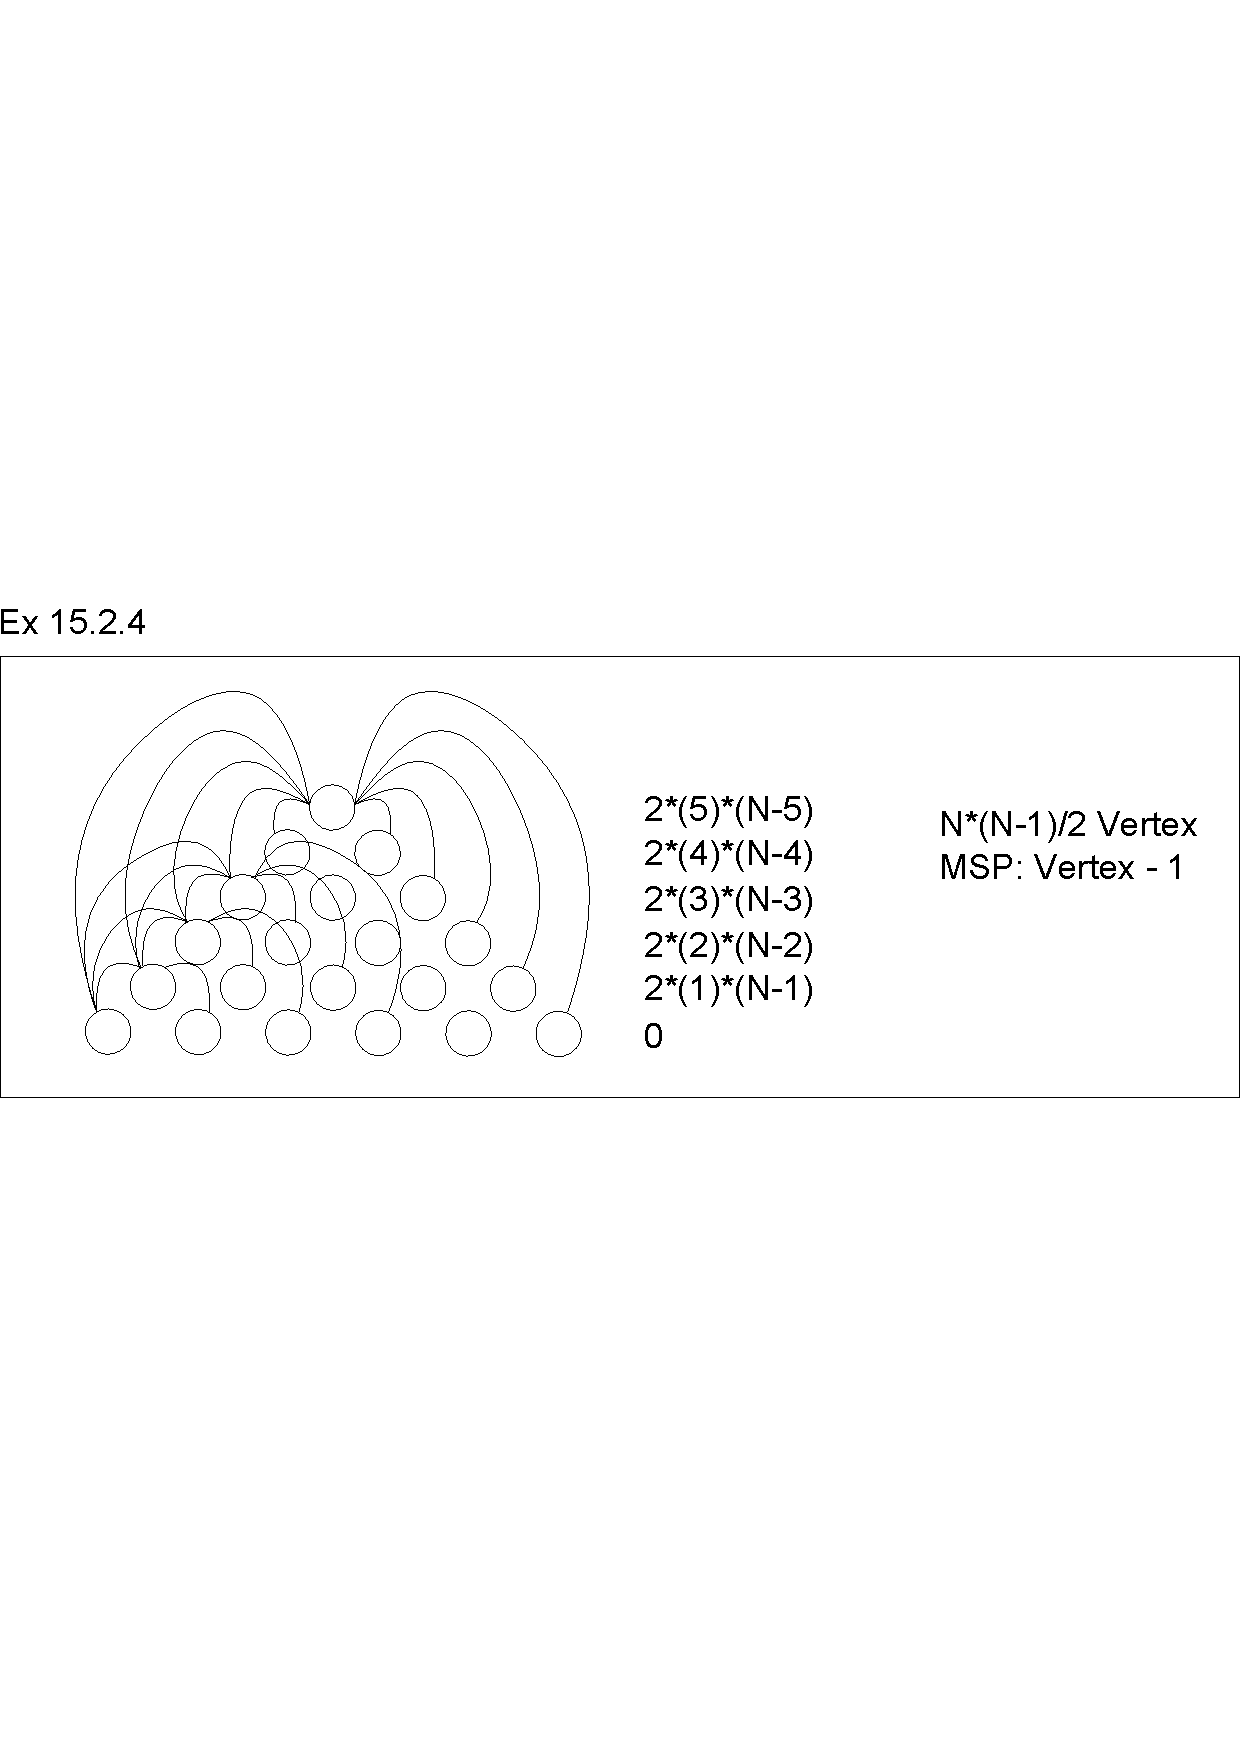
\includegraphics[width=0.8\linewidth]{1524}
	\caption{15.2-4}
	\label{fig:15.2-4}
\end{figure}

\subsection{15.2-5}
For each level $h(i) = i (n-i)$\\
For tree $T(n) = 2\Sigma_{i = 1}^{n-1}i(n-i)
\\ = \frac{3n^3 + 3n^2}{3} - \frac{2n^3 + 3n^2 +n}{3}
\\ = \frac{n^3 - n }{3}$

\subsection{15.2-6}
Assume that $\forall k \le n-1, N(k) = k-1$\\
Then $N(n) = N(n-1) + 1$\\
So $N(n) = n-1$

\subsection{15.3-1}
running through: $T(n) = n*P_{n}^{n} = n*n! > 4^{n}$\\
running recursion: $T(n) = 2\Sigma_{i=1}^{n-1}4^i + n = \frac{8}{3}4^{n-1} + n \le 4^n$\\
running through takes longer

\subsection{15.3-2}
no overlapping subproblem call

\subsection{15.3-3}
Yes

\subsection{15.3-4}
Do not know how!

\subsection{15.4-1}
See code

\subsection{15.4-2}
See code

\subsection{15.4-3}
See code


\end{document}
